\documentclass[11pt,a4paper]{article}
% ============================================================
% Shared preamble for Claude Experiments reports (pdflatex)
% Include this AFTER \documentclass in each report:
%   \documentclass[11pt,a4paper]{article}
%   % ============================================================
% Shared preamble for Claude Experiments reports (pdflatex)
% Include this AFTER \documentclass in each report:
%   \documentclass[11pt,a4paper]{article}
%   % ============================================================
% Shared preamble for Claude Experiments reports (pdflatex)
% Include this AFTER \documentclass in each report:
%   \documentclass[11pt,a4paper]{article}
%   \input{../preamble}
% ============================================================
\usepackage[T1]{fontenc}
\usepackage[utf8]{inputenc}
\usepackage[english]{babel}
\usepackage[a4paper,top=2.5cm,bottom=2.5cm,left=2.5cm,right=2.5cm]{geometry}
\usepackage{amsmath,amssymb}
\usepackage{graphicx}
\usepackage{subcaption}
\usepackage{booktabs}
\usepackage{xcolor}
\usepackage[colorlinks=true,allcolors=blue]{hyperref}
\usepackage{microtype}
\usepackage{float}
\usepackage{array}
\microtypesetup{expansion=false}

% Color scheme
\definecolor{colMicro}{HTML}{222222}
\definecolor{colExact}{HTML}{2878b5}
\definecolor{colPlacement}{HTML}{e07a1f}
\definecolor{colBoundary}{HTML}{429c74}
\definecolor{colCurrent}{HTML}{c23b55}
\definecolor{colMM}{HTML}{c23b55}

\providecommand{\SIG}{\textcolor{green!50!black}{\textbf{*}}}
\providecommand{\NS}{\textcolor{gray}{n.s.}}
\providecommand{\DRMS}{\Delta\mathrm{RMST}}
\providecommand{\ci}[2]{$[{#1},\;{#2}]$}

% ============================================================
\usepackage[T1]{fontenc}
\usepackage[utf8]{inputenc}
\usepackage[english]{babel}
\usepackage[a4paper,top=2.5cm,bottom=2.5cm,left=2.5cm,right=2.5cm]{geometry}
\usepackage{amsmath,amssymb}
\usepackage{graphicx}
\usepackage{subcaption}
\usepackage{booktabs}
\usepackage{xcolor}
\usepackage[colorlinks=true,allcolors=blue]{hyperref}
\usepackage{microtype}
\usepackage{float}
\usepackage{array}
\microtypesetup{expansion=false}

% Color scheme
\definecolor{colMicro}{HTML}{222222}
\definecolor{colExact}{HTML}{2878b5}
\definecolor{colPlacement}{HTML}{e07a1f}
\definecolor{colBoundary}{HTML}{429c74}
\definecolor{colCurrent}{HTML}{c23b55}
\definecolor{colMM}{HTML}{c23b55}

\providecommand{\SIG}{\textcolor{green!50!black}{\textbf{*}}}
\providecommand{\NS}{\textcolor{gray}{n.s.}}
\providecommand{\DRMS}{\Delta\mathrm{RMST}}
\providecommand{\ci}[2]{$[{#1},\;{#2}]$}

% ============================================================
\usepackage[T1]{fontenc}
\usepackage[utf8]{inputenc}
\usepackage[english]{babel}
\usepackage[a4paper,top=2.5cm,bottom=2.5cm,left=2.5cm,right=2.5cm]{geometry}
\usepackage{amsmath,amssymb}
\usepackage{graphicx}
\usepackage{subcaption}
\usepackage{booktabs}
\usepackage{xcolor}
\usepackage[colorlinks=true,allcolors=blue]{hyperref}
\usepackage{microtype}
\usepackage{float}
\usepackage{array}
\microtypesetup{expansion=false}

% Color scheme
\definecolor{colMicro}{HTML}{222222}
\definecolor{colExact}{HTML}{2878b5}
\definecolor{colPlacement}{HTML}{e07a1f}
\definecolor{colBoundary}{HTML}{429c74}
\definecolor{colCurrent}{HTML}{c23b55}
\definecolor{colMM}{HTML}{c23b55}

\providecommand{\SIG}{\textcolor{green!50!black}{\textbf{*}}}
\providecommand{\NS}{\textcolor{gray}{n.s.}}
\providecommand{\DRMS}{\Delta\mathrm{RMST}}
\providecommand{\ci}[2]{$[{#1},\;{#2}]$}

\title{CE-10: Spectral Correction Ladder}
\author{Two-Layer CTMC Experiments Pipeline}
\date{August 4, 2026}
\begin{document}\maketitle
\begin{abstract}
CE-10 evaluates the parameters-only spectral exponent $\alpha=\mathrm{clamp}(1/\mu_2,1,6)$ across export ratios and internal degrees. The correction is effective in the fast-export regime but systematically harmful when export is slow, where the uncorrected model is already near zero or late. Seven of twelve cells improved, with gap closure up to 0.93, while five regressed and the worst low-$r$ cell amplified error more than sevenfold. Spectral damping is therefore a useful component only behind a regime-aware activation gate.
\end{abstract}
\section{Design}
The 12-cell grid used $r\in\{0.5,1,2\}$, $d\in\{4,6,10,20\}$, $k=5$, and 60 paired replications. Each replication shared Full Micro, network, initialization, and nominal seed between baseline and corrected MicroMacro. Gap closure is $(|\Delta RMST_{off}|-|\Delta RMST_{spectral}|)/|\Delta RMST_{off}|$.

\section{Results}
\begin{table}[H]\centering
\caption{Means over four degree cells.}
\begin{tabular}{rrrr}\toprule
$r$ & Off normalized error & Spectral normalized error & Mean gap closure\\\midrule
0.5&-0.0128& 0.1262&-3.381\\
1.0&-0.1265& 0.0960& 0.403\\
2.0&-0.2879& 0.0055& 0.675\\
\bottomrule\end{tabular}
\end{table}
The best cell was $(r,d)=(2,6)$ with gap closure 0.933. The worst was $(0.5,10)$ at $-7.095$. At $r=1$, performance transitions from regression at low degree to strong improvement at higher degree. Positive closure occurred in 7 of 12 cells.
\begin{figure}[H]\centering
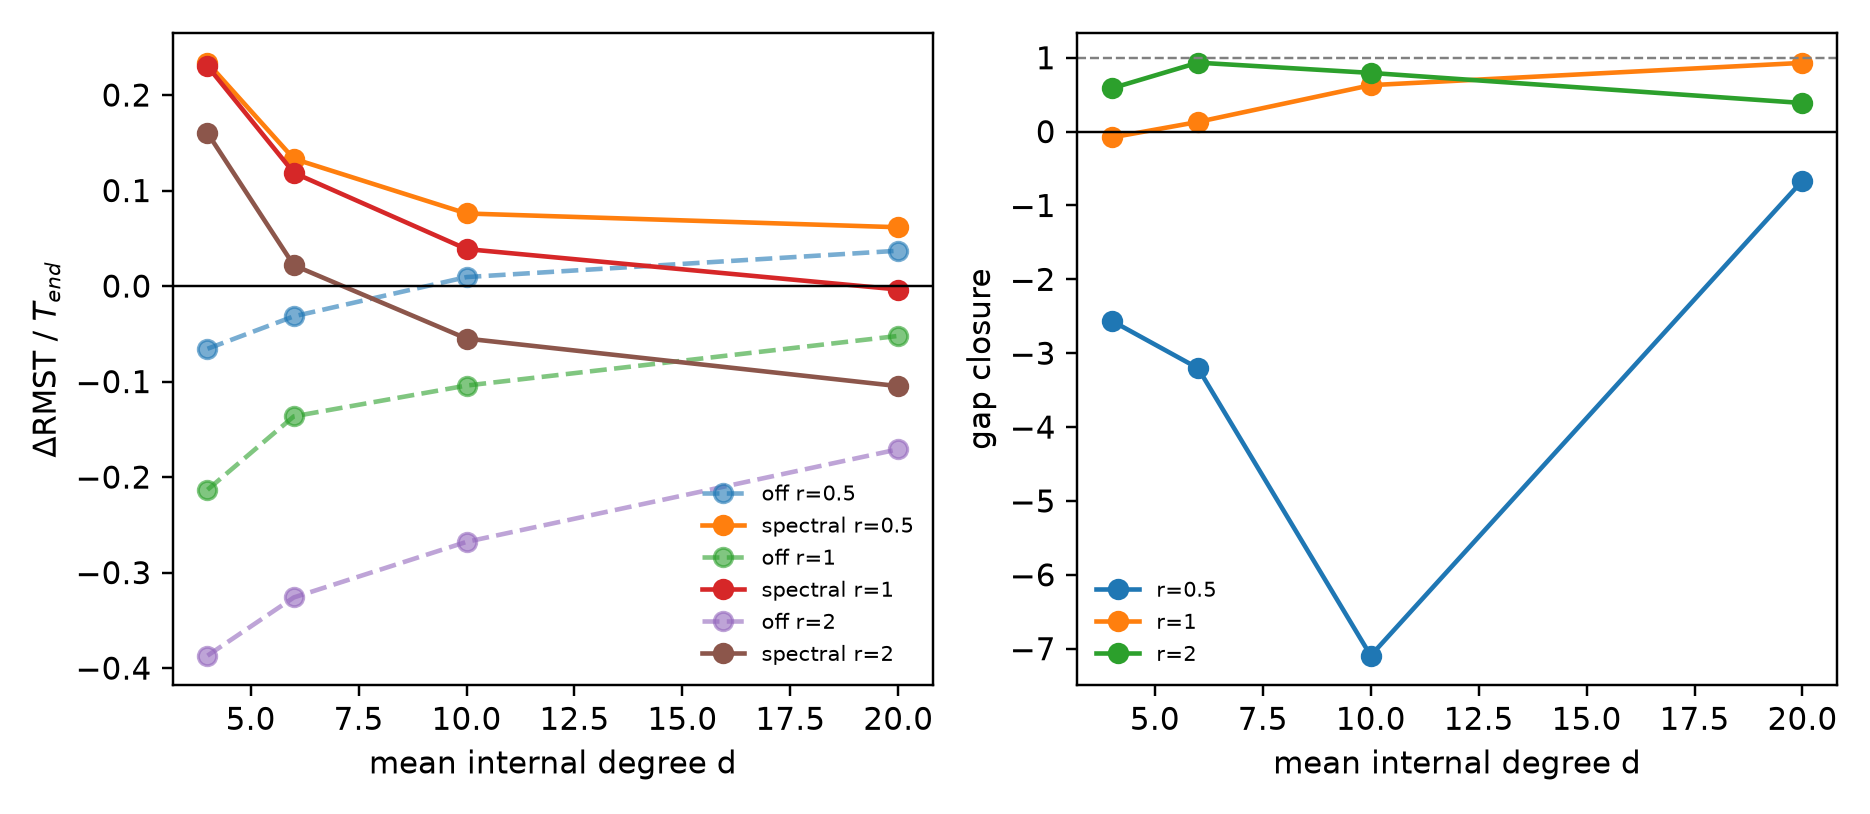
\includegraphics[width=.9\linewidth]{figures/spectral_correction.png}
\caption{Normalized timing error and gap closure. Each point summarizes 60 paired replications.}
\end{figure}

\section{Implications for correction design}
The experiment validates the direction of spectral damping in the regime it targets: when export competes with or exceeds internal mixing, delaying effective contagiousness can remove most premature leakage. It simultaneously rejects the correction as an always-on rule. At $r=0.5$, damping converts small mixed-sign baseline errors into large late-arrival errors.

The next candidate should combine spectral information with a sign-aware gate based on $r$ relative to mixing, and should continuously approach identity in slow-export and clique-like regimes. CE-10 also warns against optimizing mean gap closure alone: a deployable correction requires a minimax criterion that penalizes the worst topology/regime regression. The active ER-01 multi-topology pilot is the appropriate next gate.

\section{Limitations}
Only random-connected SI communities and $k=5$ are represented. The correction was evaluated on the same regime family that motivated it, so topology transfer remains unresolved. Runtime is an implementation diagnostic only.
\section*{Reproduction}
\texttt{.venv/bin/python extrascripts/run\_ce10\_correction\_ladder.py --grid full --workers 12 --resume}
\end{document}
